% mainfile: ../../../../master.tex
\subsection{DNA and RNA quantification with NanoDrop\cR ND-1000 Spectrophotometer}
% The part of the label after the colon must match the file name. Otherwise,
% conditional compilation based on task labels does NOT work.
\label{task:20180320_cj3}
\tags{lab,dna,rna,qnt}
\authors{cj}
\files{/mime/scripts/py/ndv\_to\_latex\_tab.py}
%\persons{}

\begin{figure}[H] % position of the figure 
    \centering
    \caption{NanoDrop spectra for DNA and RNA isolated with AllPrep\cR Mini Kit}
    \label{fig:label}
    \begin{subfigure}[b]{0.49\textwidth}
        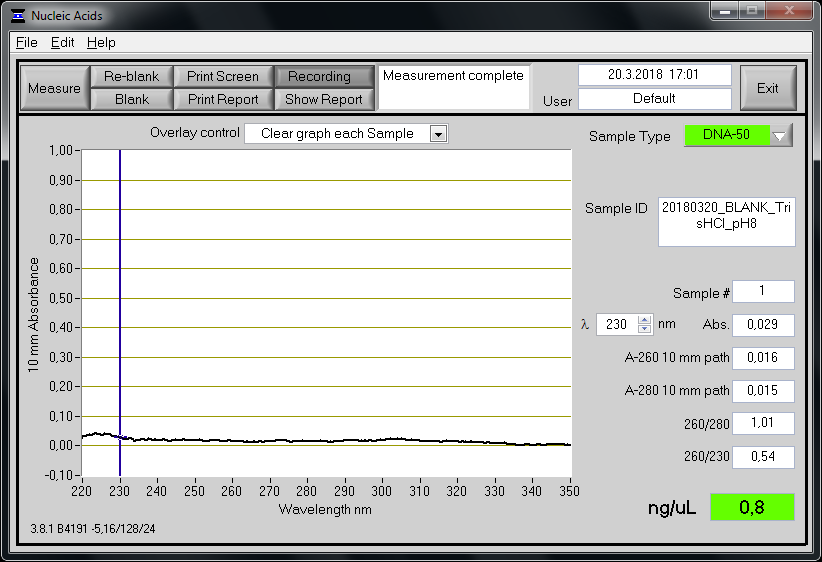
\includegraphics[width=\textwidth]{graphics/screenshots/CJ20180320_BLANK_TrisHCl_pH8.png}
        \caption{Spectrum of the Tris-HCl buffer pH 8 used as Blank}
        \label{sfig:CJ20180320_BLANK_TrisHCl_pH8}
    \end{subfigure}
    ~ 
    \begin{subfigure}[b]{0.49\textwidth}
        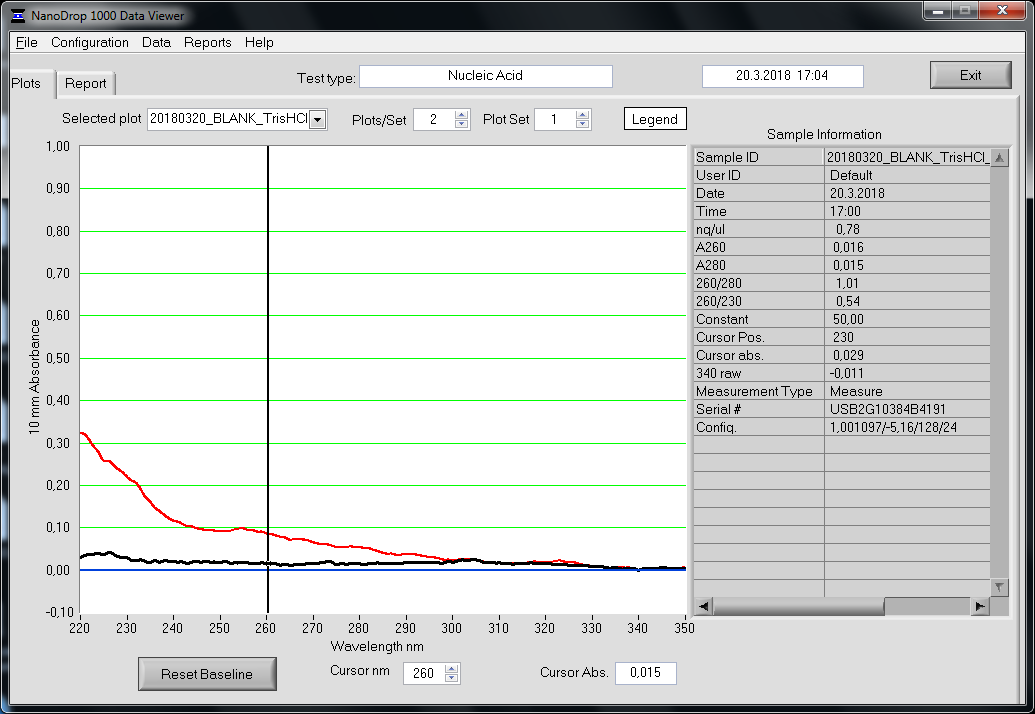
\includegraphics[width=\textwidth]{graphics/screenshots/CJ20180320_AllPrep_DNA.png}
        \caption{Spectrum of the DNA}
        \label{sfig:CJ20180320_AllPrep_DNA}
    \end{subfigure}
    \\
    \begin{subfigure}[b]{0.49\textwidth}
        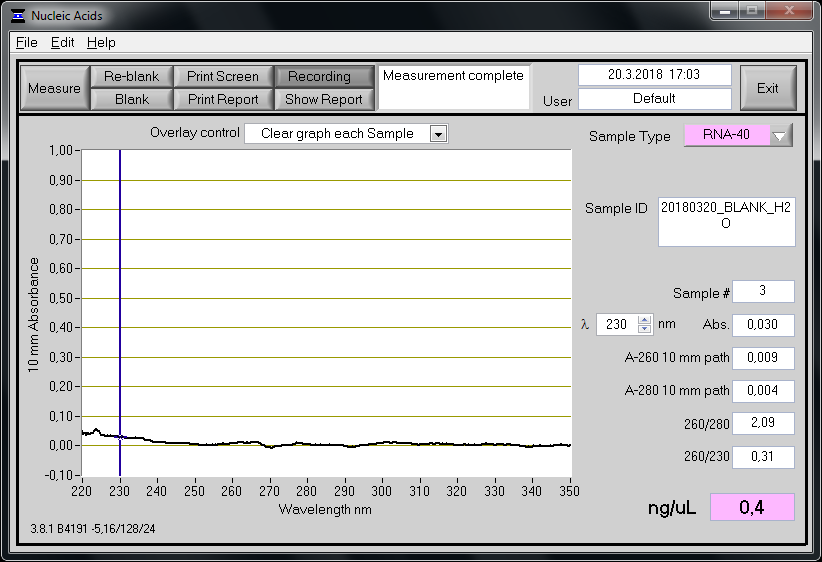
\includegraphics[width=\textwidth]{graphics/screenshots/CJ20180320_BLANK_H2O.png}
        \caption{Spectrum of the dH2O used as Blank}
        \label{sfig:CJ20180320_BLANK_H2O}
    \end{subfigure}
    ~ 
    \begin{subfigure}[b]{0.49\textwidth}
        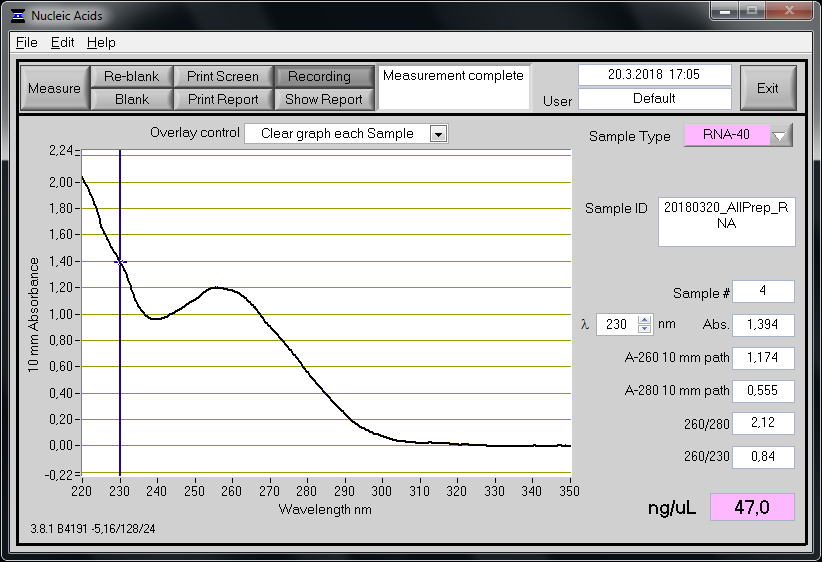
\includegraphics[width=\textwidth]{graphics/screenshots/CJ20180320_AllPrep_RNA.png}
        \caption{Spectrum of the RNA}
        \label{sfig:CJ20180320_AllPrep_RNA}
    \end{subfigure}
\end{figure}

I find that the spectrum obtained for the RNA is not too bad (cf. figure \ref{sfig:CJ20180320_AllPrep_RNA}).

\begin{table}[H]
\caption{CJ20180320.txt}
\label{tab:}
\centering
\begin{tabular}{l l l l l l l l l l l l l }
\toprule
Sample ID & Time  & ng/ul  & A260  & A280  & 260/280  & 260/230  \\ \midrule
\texttt{20180320\_BLANK\_TrisHCl\_pH8} & 17:00 & 0,78 & 0,016 & 0,015 & 1,01 & 0,54 \\
\texttt{20180320\_AllPrep\_DNA} & 17:02 & 4,28 & 0,086 & 0,054 & 1,59 & 0,39 \\
\texttt{20180320\_BLANK\_H2O} & 17:03 & 0,37 & 0,009 & 0,004 & 2,09 & 0,31 \\
\texttt{20180320\_AllPrep\_RNA} & 17:05 & 46,95 & 1,174 & 0,555 & 2,12 & 0,84 \\
\bottomrule
\end{tabular}
\\
User: Default - Date: 20.3.2018 - Constant: 40,00 - Cursor position: 230 \
\end{table}